\documentclass[12pt]{kiarticle}
\graphicspath{{pictures/}}
\DeclareGraphicsExtensions{.pdf,.png,.jpg,.eps}
\pagestyle{fancy}
\fancyhf{}
%\renewcommand{\headrulewidth}{ 0.1mm }
\renewcommand{\footrulewidth}{ .0em }
\fancyfoot[C]{\texttt{\textemdash~\thepage~\textemdash}}
\fancyhead[L]{Лабораторная работа № 123 \hfil}
\fancyhead[R]{\hfil Коляскин Дмитрий, 622 группа }
\usepackage{multirow} % Слияние строк в таблице
\newcommand
{\un}[1]
{\ensuremath{\text{#1}}}
\newcommand{\eds}{\ensuremath{ \mathscr{E}}}
\usepackage{tikz}

\begin{document}

\begin{titlepage}
	\begin{center}
		\large 	Московский физико-технический институт \\
		Факультет общей и прикладной физики \\
		\vspace{0.2cm}
		
		\vspace{4.5cm}
		Лабораторная работа № 123 \\ \vspace{0.2cm}
		\large (Общая физика: электричество и магнетизм) \\ \vspace{0.2cm}
		\LARGE \textbf{Резонанс токов в параллельном контуре}
	\end{center}
	\vspace{2.3cm} \large
	
	\begin{center}
		Работу выполнил: \\
		Коляскин Дмитрий,
		622 группа
		\vspace{10mm}		
		
	\end{center}
	
	\begin{center} \vspace{60mm}
		г. Долгопрудный \\
		2017 год
	\end{center}
\end{titlepage}



\paragraph*{Цель работы:} исследование резонанса токов в параллельном колебательном контуре с изменяемой
ёмкостью, включающее получение амплитудно-частотных и фазово-частотных характеристик, а также определение основных параметров контура.

\paragraph*{Оборудование:} генератор сигналов, источник тока, нагруженный на параллельный колебательный контур с переменной ёмкостью, двулучевой осциллограф, цифровые вольтметры.


\section{Теоретическое введение и описание установки}
\begin{figure}[h]
\begin{minipage}[h]{0.49\linewidth}
\center{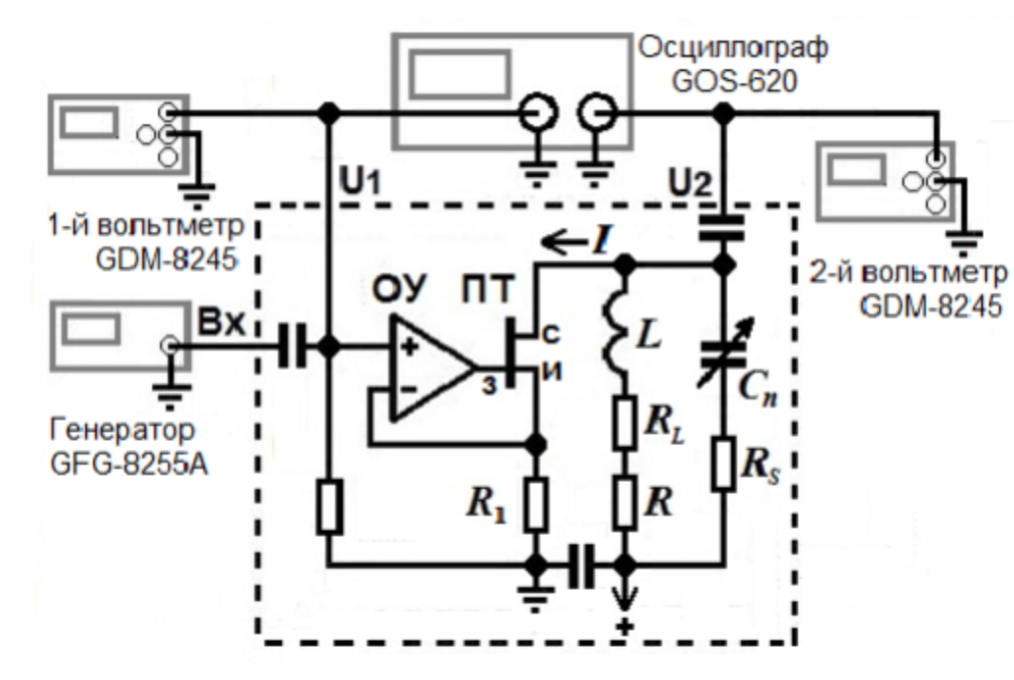
\includegraphics[width=1\linewidth]{im2} \\ Рис.1 Схема установки.}
\end{minipage}
\hfill
\begin{minipage}[h]{0.49\linewidth}
\center{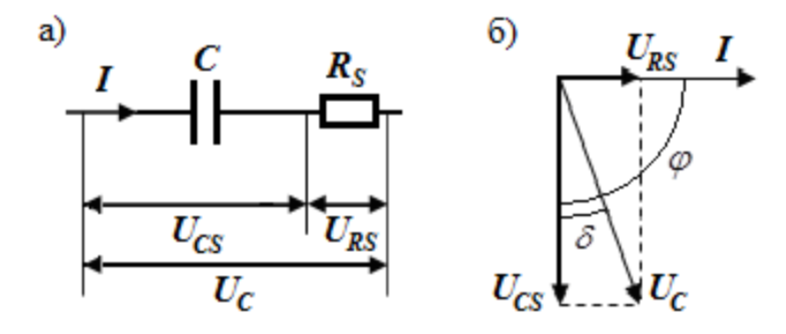
\includegraphics[width=1\linewidth]{im1} \\ Рис.2 Последовательная эквивалентная схема конденсатора с потерями.}
\end{minipage}
\end{figure}

$I=\dfrac{E}{R_I}=\dfrac{E_0cos(\omega t+\varphi_0)}{R_I}=I_0cos(\omega t+\varphi_0)$ --- ток на генераторе\newline
$$R_S=\dfrac{U_{RS}}{I}=\frac{U_{RS}}{\omega CU_{CS}}=\dfrac{1}{\omega C}tg\delta$$
где $R_S$ - эквивалентное последовательное сопротивление (ЭПС)\newline
Для используемых емкостей $C_n$ выполнено $tg\delta<10^{-3}$\newline
$$R_{\sum}=R+R_L+R_S$$
где $R_{\sum}$ - суммарное активное сопротивление контура.\newline
Воспользуемся методом комплексных амплитуд:\newline
$Z_L=R_L+i\omega L$, $Z_C=R_S-i\frac{1}{\omega C}$, $Z=R_{\sum}+i(\omega L-d\dfrac{1}{\omega C})$\newline
Тогда напряжение на контуре и токи на индуктивной и емкостной частях контура при нулевой начальной фазе можно предствить в виде:\newline
$$I_c=I\dfrac{Z_L}{Z_C+Z_L}=iQI_0\dfrac{\omega}{\omega_0}\dfrac{1-i\dfrac{R+R_L}{\rho}\dfrac{\omega_0}{\omega}}{1+iQ(\dfrac{\omega}{\omega_0}-\dfrac{\omega_0}{\omega})}$$
$$I_L=I\dfrac{Z_c}{Z_C+Z_L}=iQI_0\frac{\omega_0}{\omega}\frac{1+itg\delta}{1+iQ(\frac{\omega}{\omega_0}-\frac{\omega_0}{\omega})}$$
$$U=I\frac{Z_LZ_c}{Z_C+Z_L}=Q\rho I_0\frac{(1-i\frac{R+R_L}{\rho}\frac{\omega_0}{\omega})(1+itg\delta)}{1+iQ(\frac{\omega}{\omega_0}-\frac{\omega_0}{\omega})}$$
где $\omega_0=\frac{1}{\sqrt{LC}}$ - собственная частота, $\rho=\sqrt{\frac{L}{C}}$ - реактивное сопротивление контура, $Q=\frac{\rho} - {R_{\sum}}$ - добротность контура\newline
Рассмотрим случай, когда $|\Delta\omega|=|\omega-\omega_0|\ll\omega_0$. Тогда
$$\frac{\omega}{\omega_0}-\frac{\omega_0}{\omega}=\frac{2\Delta\omega}{\omega_0}$$
Пренебрегая поправками порядка $Q^{-2}$, получим:
$$I_c=QI_0\frac{\omega}{\omega_0}\frac{e^{i\phi_c}}{\sqrt{1+(\tau\Delta\omega)^2}},    \phi_c=\frac{\pi}{2}-\frac{R+R_L}{\rho}-arctg(\tau\Delta\omega)$$
$$I_L=QI_0\frac{\omega_0}{\omega}\frac{e^{i\phi_L}}{\sqrt{1+(\tau\Delta\omega)^2}}, \phi_L=-\frac{\pi}{2}+\delta\arctg(\tau\Delta\omega)$$
$$U=Q\rho I_0\frac{\omega}{\omega_0}\frac{e^{i\phi_U}}{\sqrt{1+(\tau\Delta\omega)^2}}, \phi_U=-\frac{\omega}{\omega_0}\frac{R+R_L}{\rho}+\delta-arctg(\tau\Delta\omega)$$
где $\tau=\frac{2L}{R_{\sum}}=\frac{2Q}{\omega_0}$ - время затухания.\newline
При резонансе, т.е. когда $\Delta\omega=0$:
$$I_c(\omega_0)=QI_0, \phi_c(\omega_0)=\frac{\pi}{2}-\frac{R+R_L}{\rho}$$
$$I_L(\omega_0)=QI_0, \phi_L(\omega_0)=-\frac{\pi}{2}+\delta$$
$$U(\omega_0)=Q\rho I_0=Q^2R_{\sum}I_0, \phi_U{\omega_0}=-\frac{R+R_L}{\rho}+\delta$$
$$\phi'_c(\omega_0)=\phi'_L(\omega_0)=\phi'_U(\omega_0)=-\tau$$


\section{Ход работы}

Данные установки: $ R = 3,50  $ Ом, $ R_1 = 1008 $ Ом.

\subsection{Измерения резонансных частот и напряжений, а также сопутствующих величин}

Проведем для 7 разных конденсаторов емкости $ C_n $ измерения резонансных частот и напряжений на них, поддерживая напряжение на вольтметре 1 равным $ E = 0,2 $ В, а также вычислим дополнительные величины, следующие из наших измерений, по следующим формулам:  

\begin{equation}\label{}
L=\frac{1}{C(2\pi f)^2} \\
\end{equation}
\begin{equation}\label{}
\rho=\frac{1}{2\pi fC} \\
\end{equation}
\begin{equation}\label{}
Z_{\text{рез}}=\frac{U}{E_0}R_1
\end{equation}
\begin{equation}\label{}
Q=\frac{UR_1}{E_0}2\pi fC
\end{equation}
\begin{equation}\label{}
R_{\sum}=\frac{E_0}{UR_1}\frac{1}{(2\pi fC)^2}
\end{equation}
\begin{equation}\label{}
R_{Smax}=10^{-3}\cdot\frac{1}{\omega_0C}
\end{equation}
\begin{equation}\label{}
R_L=\frac{E_0}{UR_1}\frac{1}{(2\pi fC)^2}-R-10^{-3}\cdot\frac{1}{\omega_0C}
\end{equation}

Результаты занесём в таблицу: 

\begin{table}[h!]
	\centering
	\caption{Результаты измерений при $ E = 0,2 \; Ом $}
\begin{tabular}{|c|c|c|c|c|c|c|c|c|c|c|}
	\hline
	$ C_n, нФ $ & $ f_{0n} $, кГц & $ U_{0n}, $ B & $ E $, B & $ L $, мкГн & $ \rho $, Ом & $ Z_{рез} $, Ом & $ Q $ & $ R_\Sigma,  $ Ом & $ R_{Sm} $, Ом & $ R_L $, Ом \\
	\hline
25.1 & 32.1 & 1.18 & 0.2 & 980.4 & 197.6 & 5947.2 & 30.1 & 6.57 & 0.20 & 2.9 \\
33.2 & 27.8 & 0.91 & 0.2 & 988.2 & 172.5 & 4586.4 & 26.6 & 6.49 & 0.17 & 2.8 \\
47.3 & 23.2 & 0.67 & 0.2 & 996.0 & 145.1 & 3376.8 & 23.3 & 6.24 & 0.15 & 2.6 \\
57.4 & 21.3 & 0.57 & 0.2 & 973.7 & 130.2 & 2872.8 & 22.1 & 5.90 & 0.13 & 2.3 \\
67.5 & 19.5 & 0.48 & 0.2 & 987.9 & 121.0 & 2419.2 & 20.0 & 6.05 & 0.12 & 2.4 \\
82.7 & 17.7 & 0.40 & 0.2 & 978.7 & 108.8 & 2016.0 & 18.5 & 5.87 & 0.11 & 2.3 \\
101.6 & 16.0 & 0.34 & 0.2 & 974.9 & 98.0 & 1713.6 & 17.5 & 5.60 & 0.10 & 2.0 \\
	\hline
	\multicolumn{4}{|c|}{Среднее значение} & 982,8 & & & & & & 2,5\\
	\multicolumn{4}{|c|}{Ср-кв. погр. ср. значения} & 2,67 & & & & & &0,10 \\
	\multicolumn{4}{|c|}{Cлучайная погрешность} & 6,3 & & & & & & 0,2\\
	\hline
\end{tabular}
	\label{resC1}% 
\end{table}% 

Теперь проведем аналогичные вычисления при $ E = 0,37 $ В.

\begin{table}[h!]
	\centering
	\caption{Результаты измерений при $ E = 0,37 \; Ом $}
	\begin{tabular}{|c|c|c|c|c|c|c|c|c|c|c|}
		\hline
		$ C_n, нФ $ & $ f_{0n} $, кГц & $ U_{0n}, $ B & $ E $, B & $ L $, мкГн & $ \rho $, Ом & $ Z_{рез} $, Ом & $ Q $ & $ R_\Sigma,  $ Ом & $ R_{Sm} $, Ом & $ R_L $, Ом \\
		\hline
25.1 & 32.1 & 2.18 & 0.37 & 980.4 & 197.6 & 5939.0 & 30.1 & 6.58 & 0.20 & 2.9 \\
33.2 & 27.8 & 1.62 & 0.37 & 988.2 & 172.5 & 4413.4 & 25.6 & 6.74 & 0.17 & 3.1 \\
47.3 & 23.2 & 1.23 & 0.37 & 996.0 & 145.1 & 3350.9 & 23.1 & 6.28 & 0.15 & 2.6 \\
57.4 & 21.3 & 1.04 & 0.37 & 973.7 & 130.2 & 2833.3 & 21.8 & 5.99 & 0.13 & 2.4 \\
67.5 & 19.5 & 0.88 & 0.37 & 987.9 & 121.0 & 2397.4 & 19.8 & 6.10 & 0.12 & 2.5 \\
82.7 & 17.7 & 0.74 & 0.37 & 978.7 & 108.8 & 2016.0 & 18.5 & 5.87 & 0.11 & 2.3 \\
101.6 & 16.0 & 0.62 & 0.37 & 974.9 & 98.0 & 1689.1 & 17.2 & 5.68 & 0.10 & 2.1 \\
		\hline
		\multicolumn{4}{|c|}{Среднее значение} & 982,8 & & & & & & 2,5\\
		\multicolumn{4}{|c|}{Ср-кв. погр. ср. значения} & 2,67 & & & & & &0,11 \\
		\multicolumn{4}{|c|}{Cлучайная погрешность} & 6,3 & & & & & & 0,3\\
		\hline
	\end{tabular}
	\label{resC2}% 
\end{table}% 

\subsection{Измерение АЧХ}

Теперь измерим амплитудно-частотную характеристику для конденсаторов $ C_2, C_5 $. При этом посчитаем также измеряемые величины по отношению к резонансным $ U_0, f_0 $. Результаты сведем в таблицу:

\begin{table}[h!]
	\centering
	\caption{Результаты измерений АЧХ}
\begin{tabular}{|c|c|c|c|c|c|c|c|c|c|}
 \hline 
 
	1 & 0.1 & 38 & 62 & 88 & 107 & 125 & 150 & 191 & 268 \\
	2 & 0.3 & 27 & 41 & 57 & 69 & 83 & 100 & 124 & 334 \\
	3 & 0.6 & 8 & 10 & 13 & 17 & 18 & 23 & 32 & 432 \\
	4 & 0.9 & -9 & -15 & -20 & -28 & -28 & -34 & -42 & 517 \\
	5 & 1.2 & -22 & -34 & -49 & -60 & -68 & -81 & -104 & 582 \\
	6 & 1.5 & -30 & -48 & -67 & -82 & -94 & -114 & -144 & 629 \\
	7 & 1.8 & -36 & -56 & -89 & -96 & -112 & -135 & -169 & 658 \\
	8 & 2.1 & -40 & -62 & -88 & -106 & -123 & -146 & -184 & 674 \\
	\hline
	\end{tabular}
	\label{resF}% 
\end{table}% 

По результатам построим графики АЧХ для обоих конденсаторов в осях $ U(f) $ и $ \dfrac{U}{U_0} \left( \dfrac{f}{f_0} \right) $.

\begin{figure}[h!]
	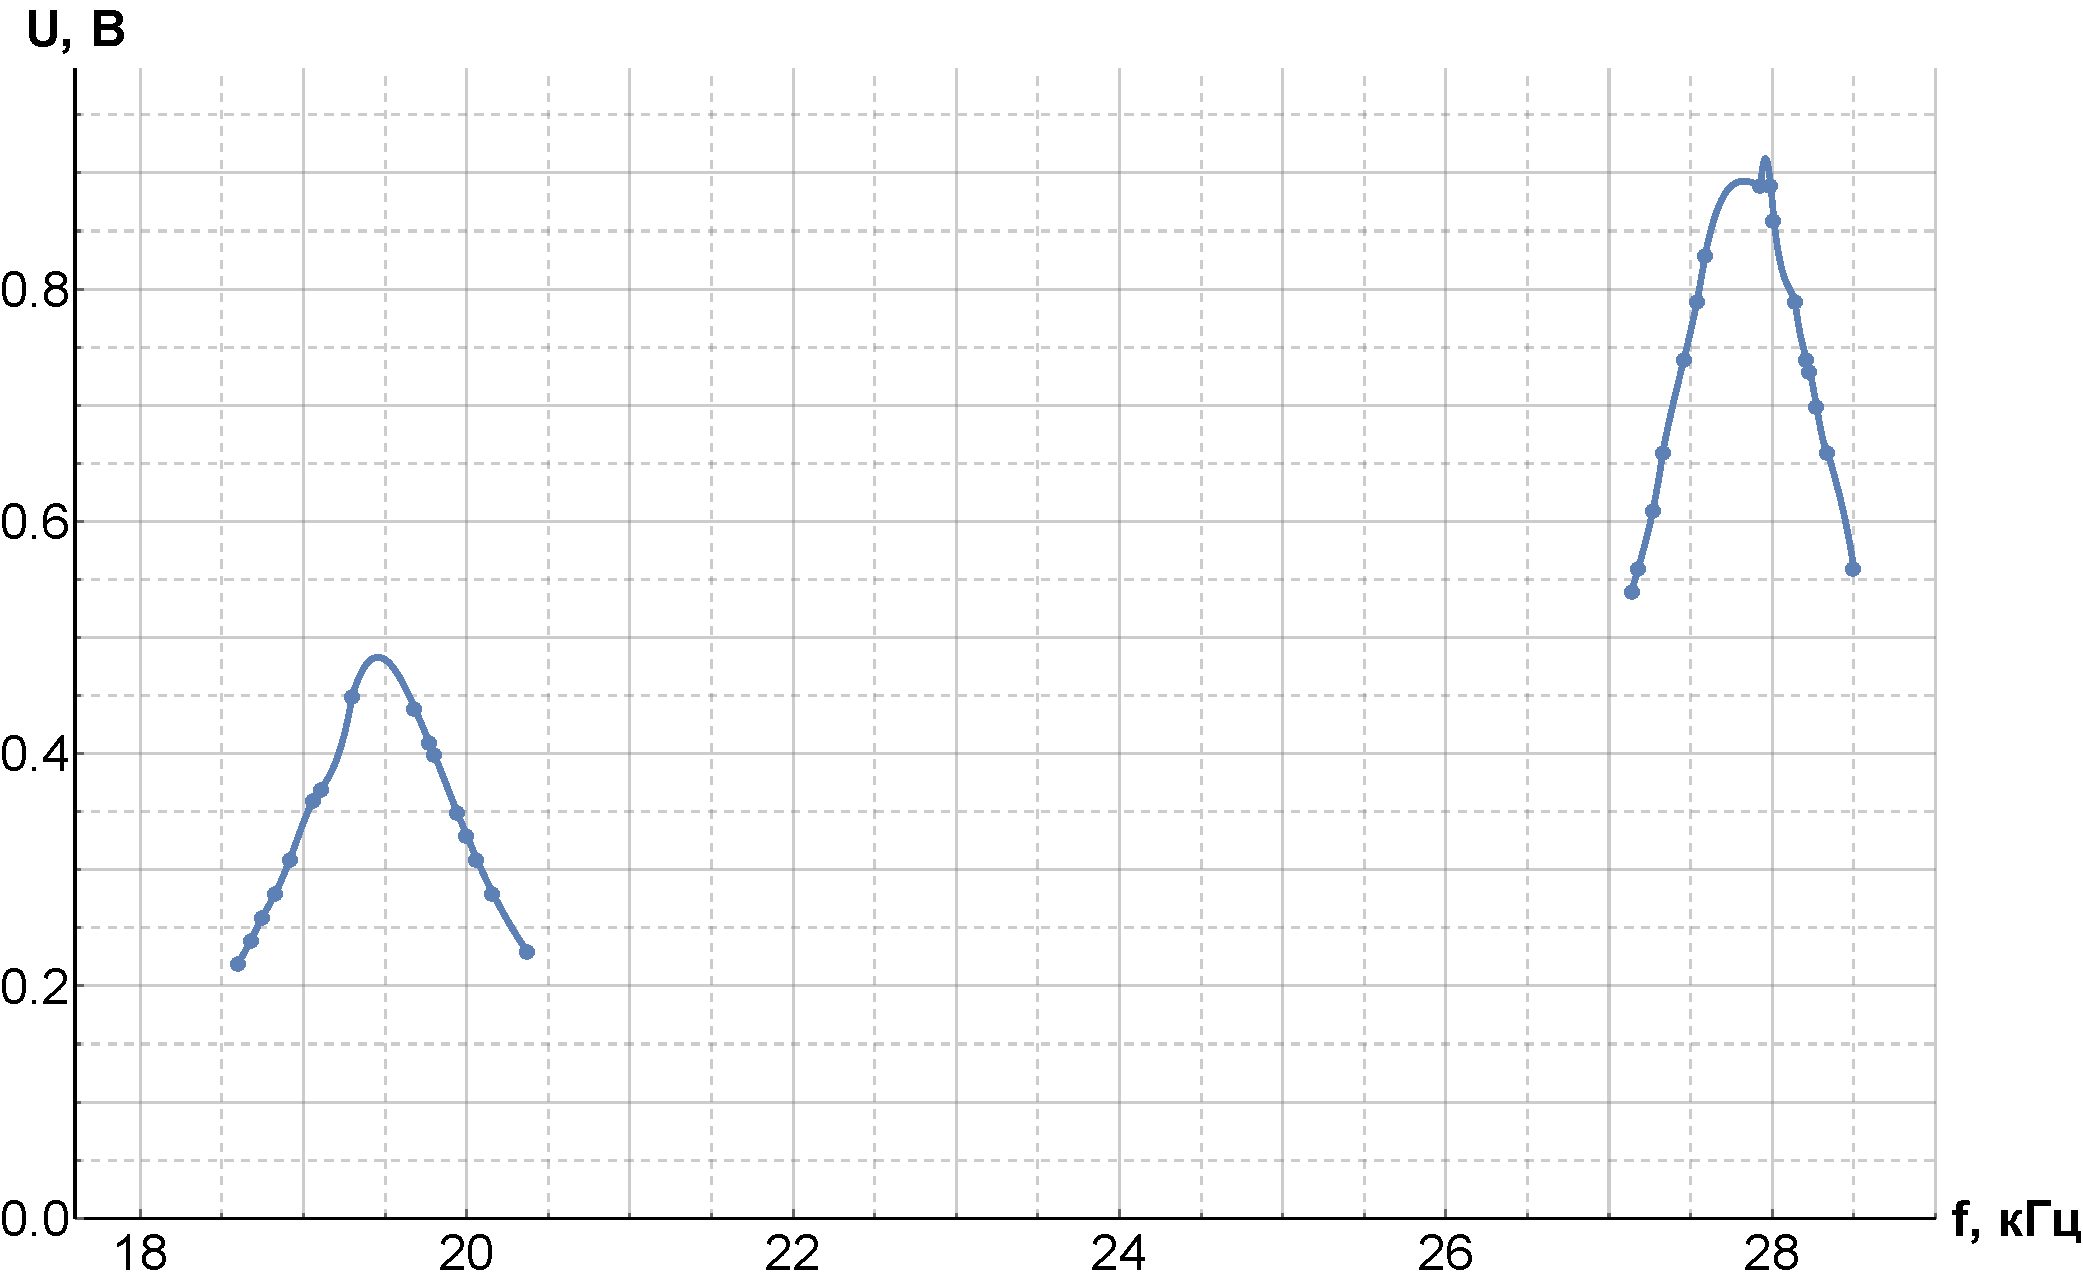
\includegraphics[scale=0.5]{F.pdf}
	\caption{График амплитудно-частотной характеристики в осях $ U(f) $ }
\end{figure}

\begin{figure}[h!]
	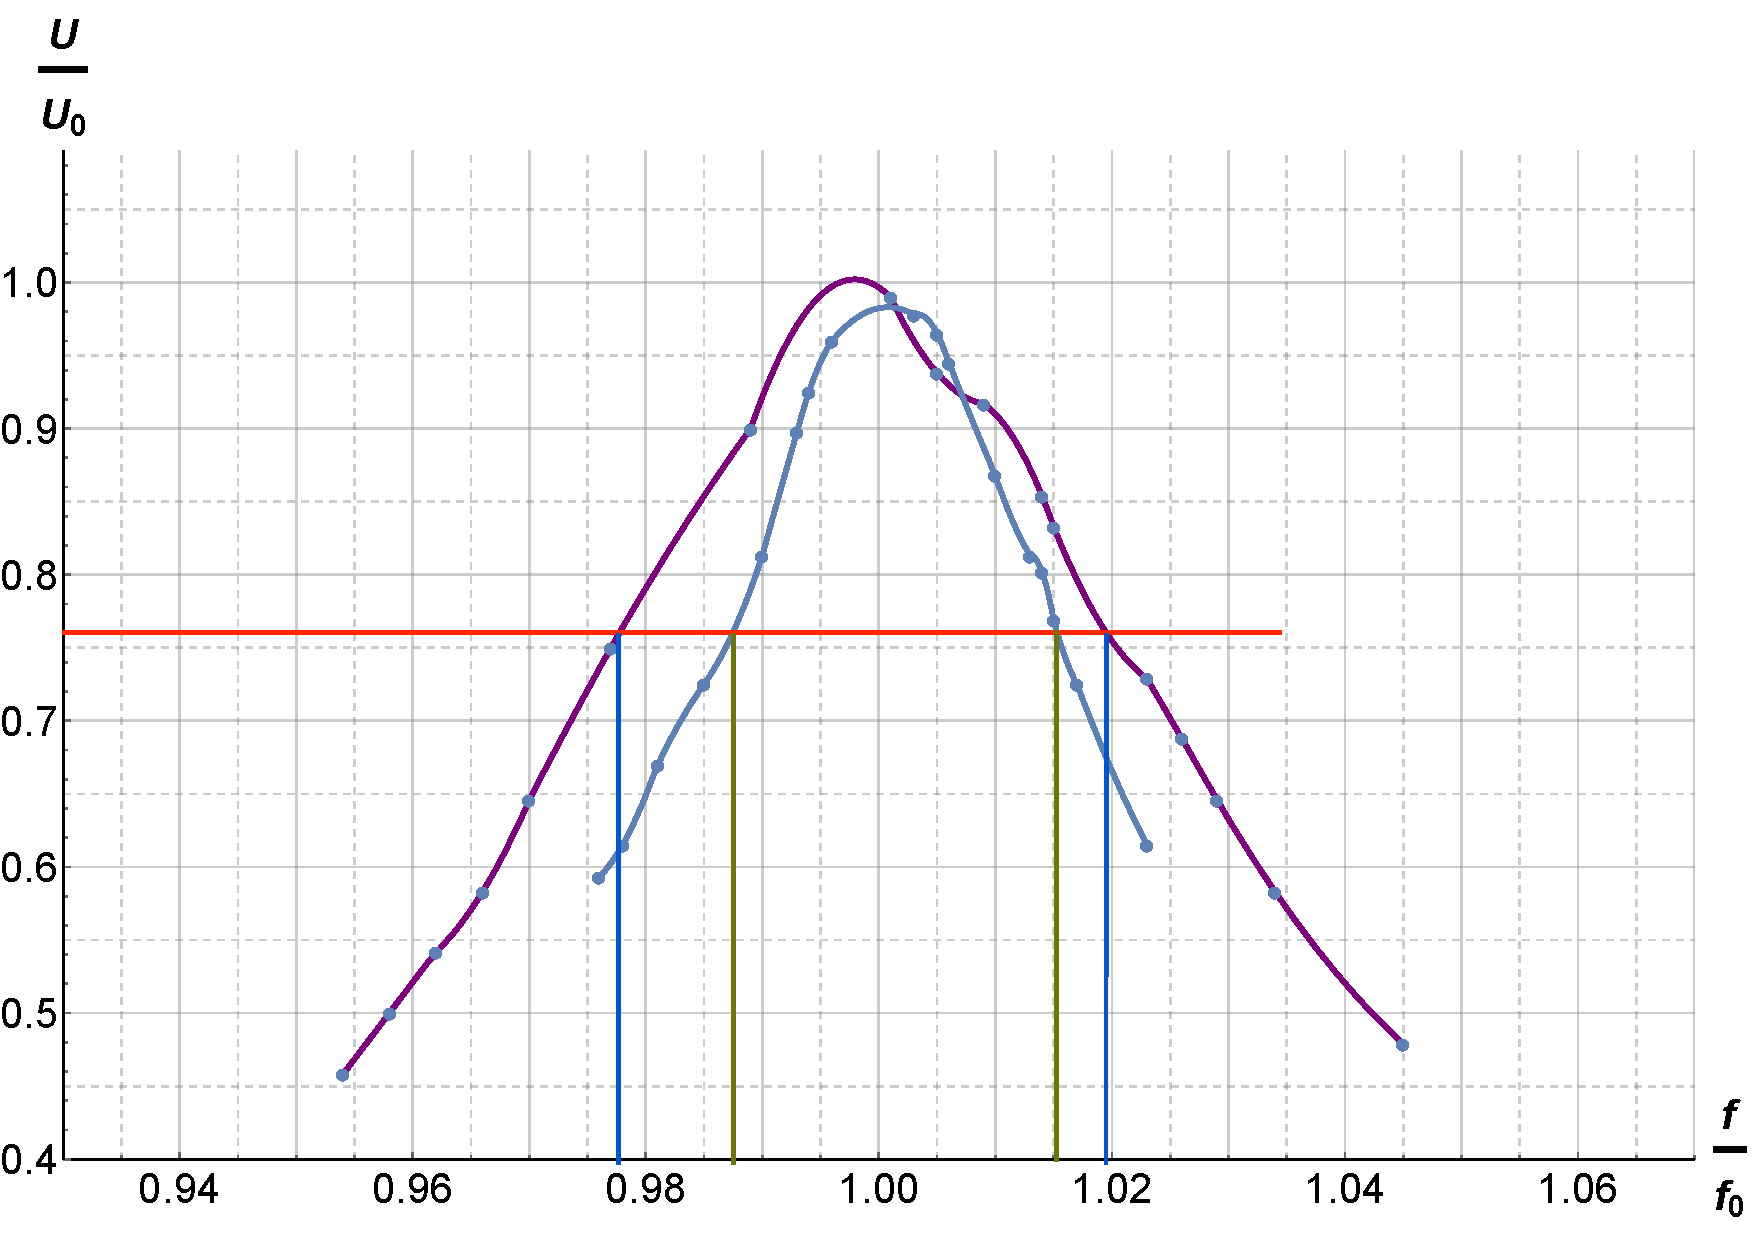
\includegraphics[scale=0.5]{fff.pdf}
	\caption{График амплитудно-частотной характеристики в осях $ \dfrac{U}{U_0} \left( \dfrac{f}{f_0} \right) $ }
\end{figure}

Теперь найдем добротность по ширине резонансной кривой $ \delta\omega $ на 2 графике как 

\begin{equation}\label{}
Q = \dfrac{1}{\delta\omega}
\end{equation}  

Где $ \delta\omega $ --- расстояние между частотами при значении напряжения $ \dfrac{1}{\sqrt{2}} $.

Получаем ответ: 

\begin{equation}\label{}
Q_2 \approx 25,9 \qquad Q_5 \approx 19,7
\end{equation}

\subsection{Фазово-частотная характеристика}

Для тех же кондесаторов определим фазово-частотную характеристику. Будем определять разность фаз между сигналами $ U(t), E(t) $ как $ \Delta\phi = \dfrac{x}{x_0}\phi $, где $ x, x_0 $ --- расстояния от начала отсчёта до момента обращения графиков этих значений в нуль. Результаты занесем в таблицу:

\begin{table}[h!]
	\centering
	\caption{Результаты измерений ФЧХ}
	\begin{tabular}{|c|c|c|c|c|c|c|c|c|c|c|}
		\hline
		\multicolumn{5}{|c|}{$ C_2 = 33,2 $ нФ} & &\multicolumn{5}{|c|}{$ C_5 = 67,5 $ нФ}  \\
		\hline
		$ U $, B & $ \dfrac{f}{f_0} $ & $ x $ & $ x_0 $ & $ \Delta\phi, \pi $ &  & 	$ U $, B & $ \dfrac{f}{f_0} $ & $ x $ & $ x_0 $ & $ \Delta\phi, \pi $\\
		\hline
		0.29 & 0.949 & 2.2 & 4.0 & 0.55 & \text{} & 0.29 & 0.967 & 4.0 & 5.8 & 0.69 \\
		0.76 & 0.989 & 3.0& 3.9 & 0.77 & \text{} & 0.42 & 0.986 & 4.6 & 5.7 & 0.81 \\
		0.90 & 1.003 & 3.9 & 3.8 & 1.03 & \text{} & 0.35 & 0.976 & 4.2 & 5.7 & 0.74 \\
		0.64 & 0.983 & 2.8 & 3.9 & 0.72 & \text{} & 0.23 & 0.953 & 3.8 & 5.7 & 0.67 \\
		0.26 & 0.944 & 2.4 & 4.0 & 0.60 & \text{} & 0.18 & 0.937 & 3.6 & 5.8 & 0.62 \\
		0.38 & 0.963 & 2.5 & 4.0 & 0.63 & \text{} & 0.47 & 0.994 & 5.0 & 5.5 & 0.91 \\
		0.77 & 0.989 & 3.1 & 3.8 & 0.82 & \text{} & 0.48 & 0.998 & 5.3 & 5.4 & 0.98 \\
		0.50 & 0.974 & 2.7 & 3.9 & 0.69 & \text{} & 0.38 & 0.981 & 4.4 & 5.5 & 0.80 \\
		0.82 & 1.008 & 4.1 & 3.7 & 1.11 & \text{} & 0.44 & 1.010 & 5.9 & 5.4 & 1.09 \\
		0.28 & 1.052 & 4.9 & 3.6 & 1.36 & \text{} & 0.26 & 1.039 & 6.7 & 5.2 & 1.29 \\
		0.56 & 1.022 & 4.7 & 3.7 & 1.27 & \text{} & 0.15 & 1.074 & 7.0 & 5.0 & 1.40 \\
		0.83 & 1.008 & 4.2 & 3.7 & 1.14 & \text{} & 0.24 & 1.043 & 6.8 & 5.2 & 1.31 \\
		0.46 & 1.03 & 4.8 & 3.7 & 1.30 & \text{} & 0.42 & 1.014 & 6.1 & 5.3 & 1.15 \\
		0.60 & 1.02 & 4.6 & 3.7 & 1.24 & \text{} & 0.46 & 1.007 & 5.8 & 5.4 & 1.07 \\
		0.74 & 1.012 & 4.4 & 3.7 & 1.19 & \text{} & 0.37 & 1.020 & 6.4 & 5.3 & 1.21 \\
		\text{} & \text{} & \text{} & \text{} & \text{} & \text{} & 0.31 & 1.029 & 6.6 & 5.20 & 1.27 \\
		\hline
	\end{tabular}
	\label{resFi}% 
\end{table}% 

По данным таблицы построим график $ \dfrac{\Delta\phi}{\pi}  \left( \dfrac{f}{f_0} \right) $.

\begin{figure}[h!]
	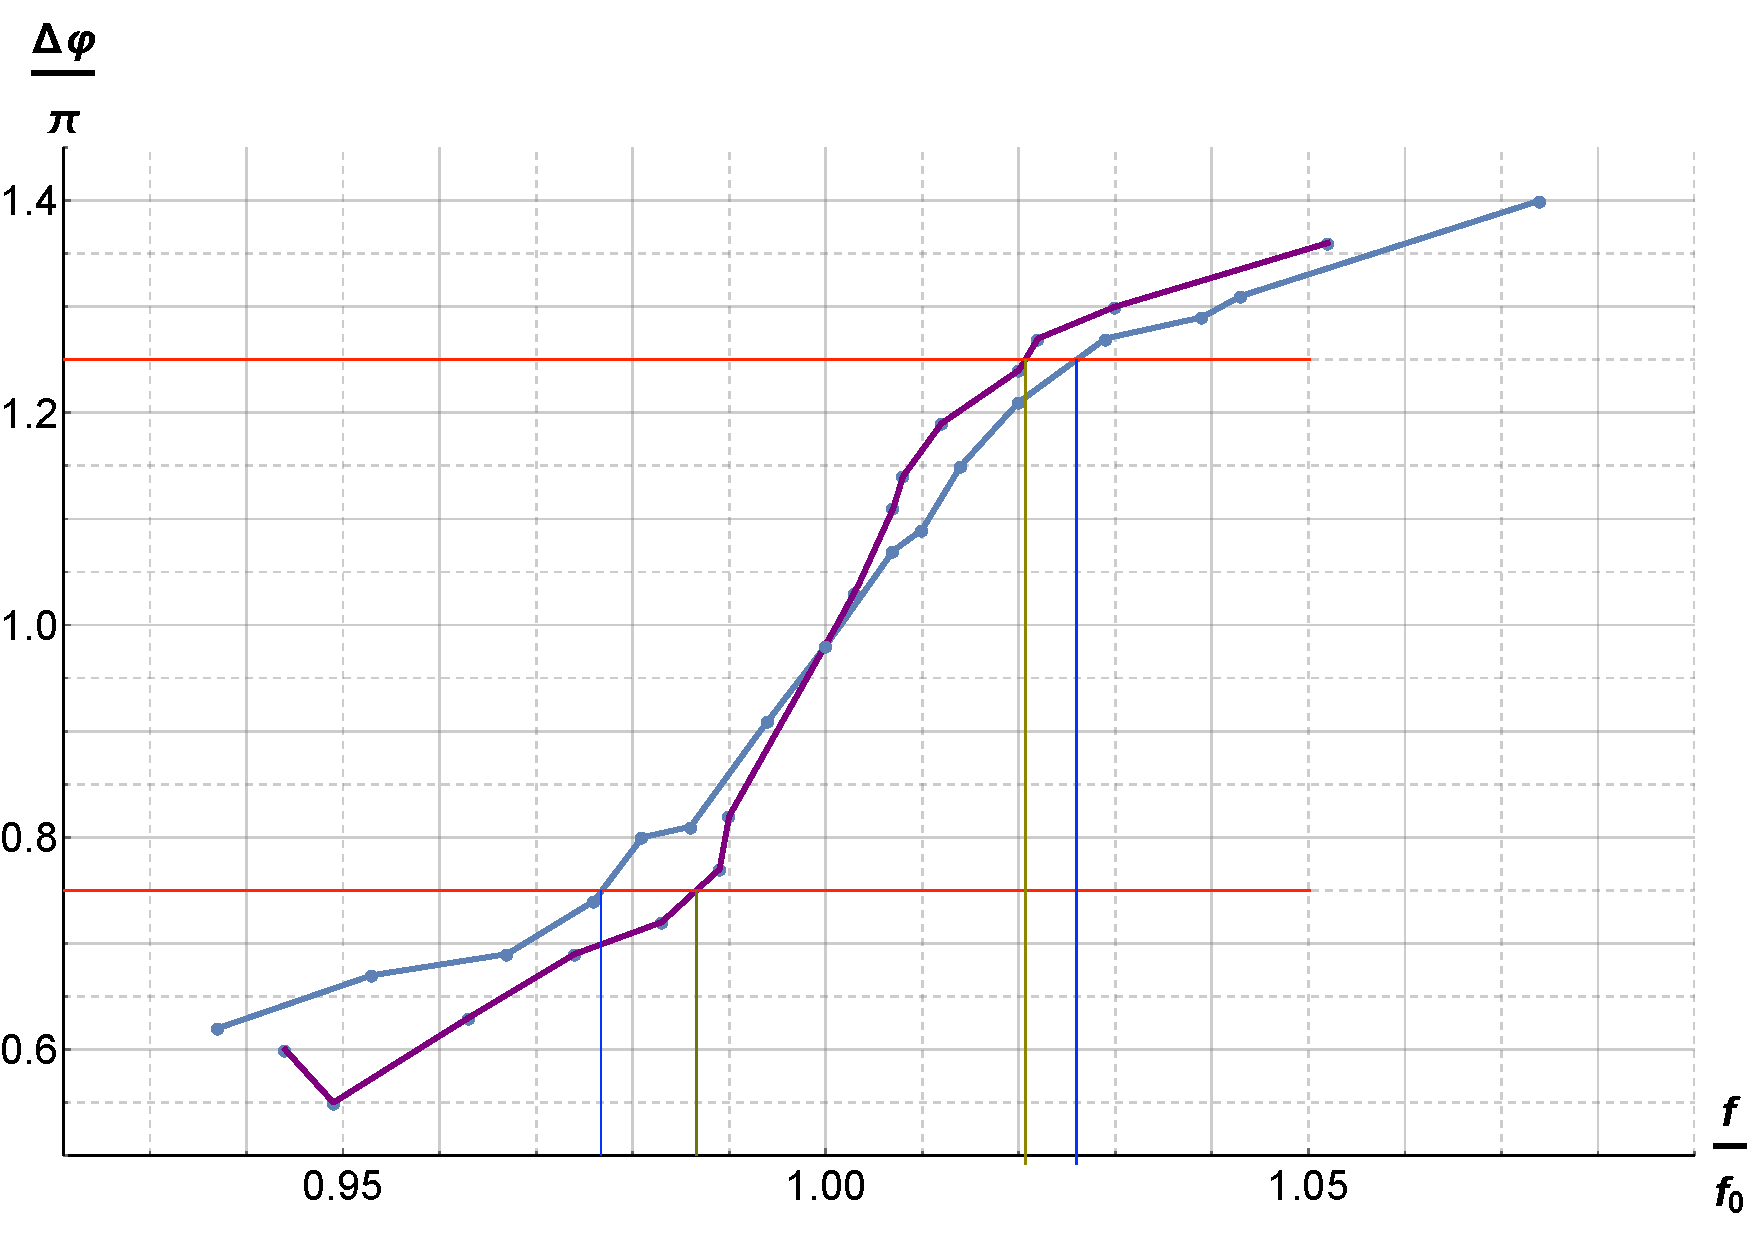
\includegraphics[scale=0.5]{Fii.pdf}
	\caption{График фазово-частотной характеристики в осях $ \dfrac{\Delta\phi}{\pi}  \left( \dfrac{f}{f_0} \right) $}
\end{figure}

Аналогично определим добротность, подсчитав длину резонансной кривой как  расстояние между частотами при разности фаз в $ \dfrac{3}{4}\pi $ и $ \dfrac{5}{4}\pi $:

\begin{equation}\label{}
Q_2 \approx 20,4 \qquad Q_5 \approx 27,1 
\end{equation}

\subsection{График  зависимости $ R_L $ от $ f_{0n} $} 

Теперь построим график зависимости $ R_L (f_{0n}) $ и проведем прямую $ \langle R_L \rangle = 2,5 $ Ом. 

\begin{figure}[h!]
	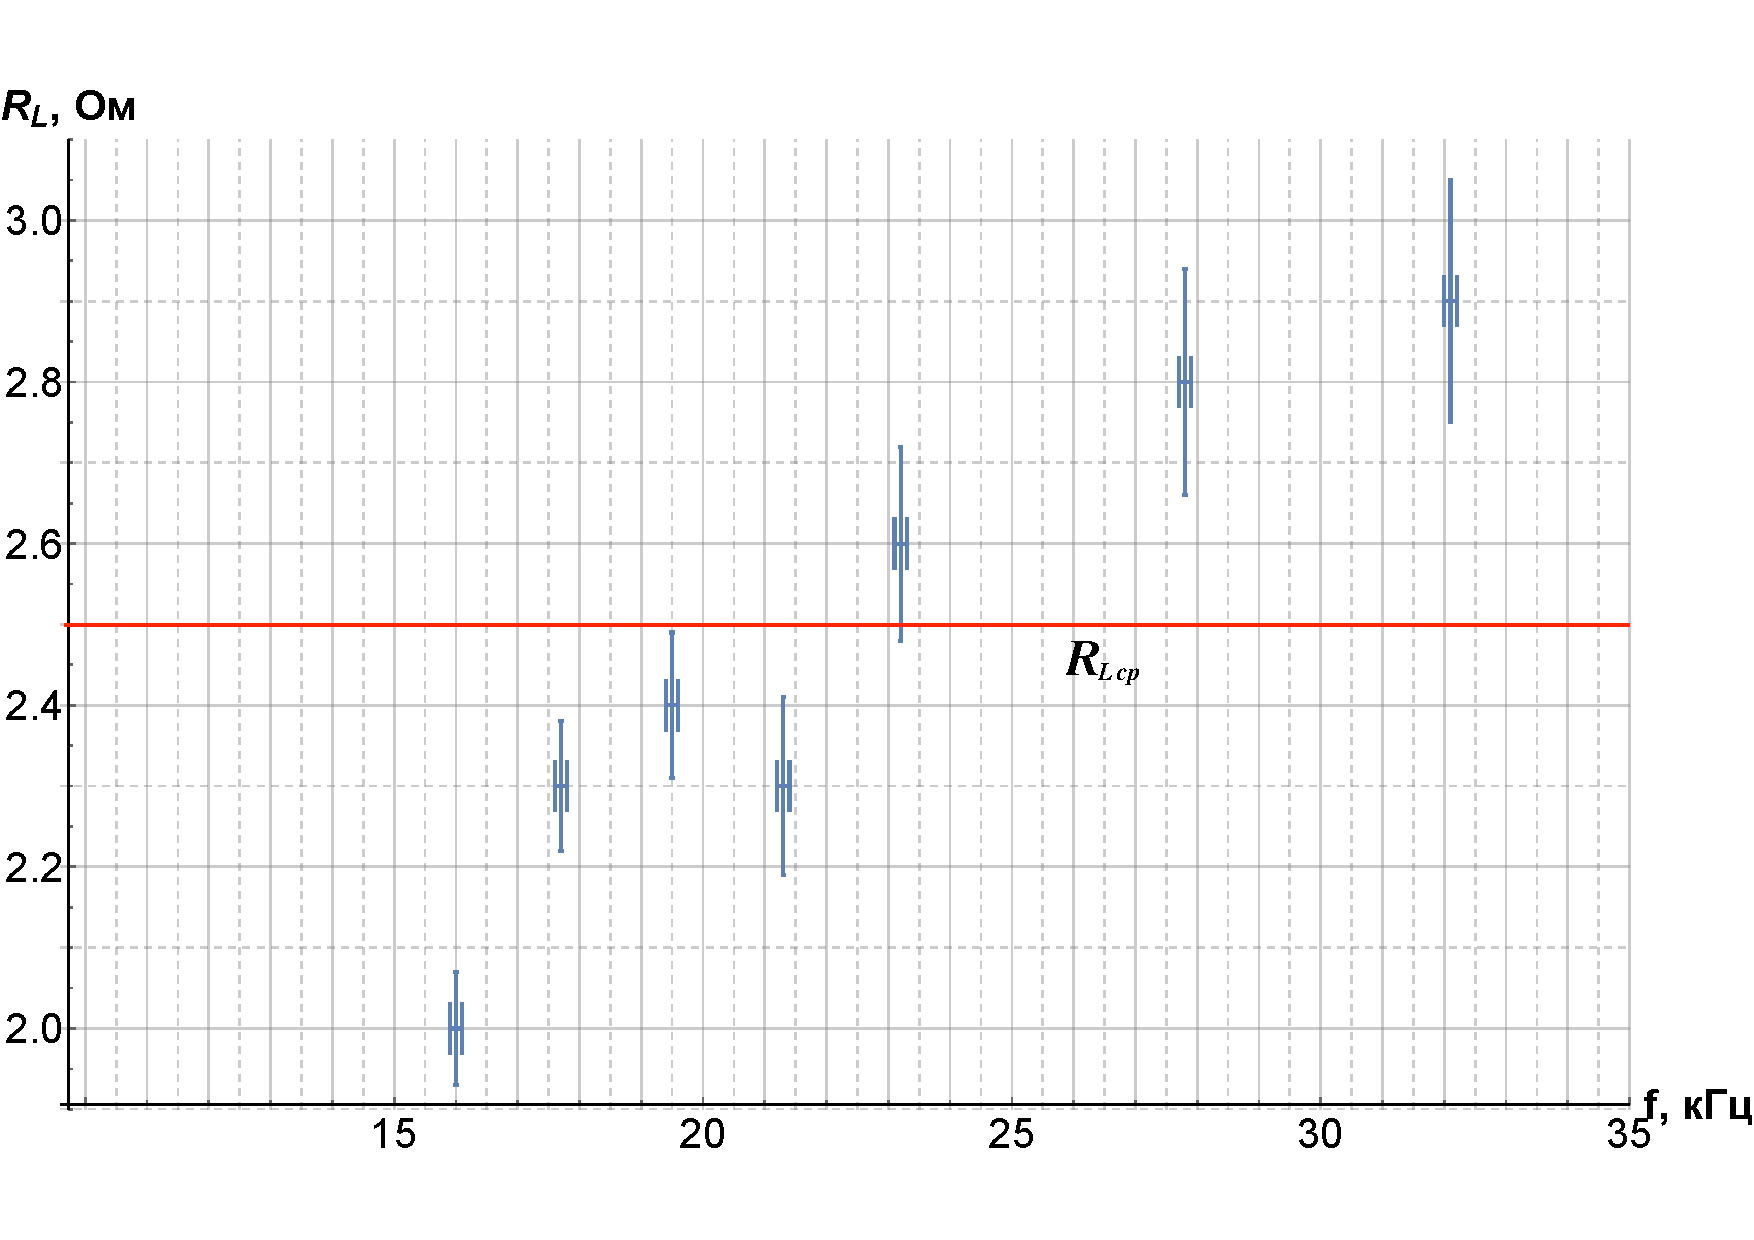
\includegraphics[scale=0.5]{RR.pdf}
	\caption{График зависимости $ R_L (f_{0n}) $}
\end{figure}
 
Видно, что $ R_L$ возрастает при увеличении частоты. Это может быть объяснено скин-эффектом. 

\newpage

\subsection{Векторная диаграмма}

Теперь построим векторную диаграмму для контура с наименьшей добротностью, т.е. для последнего --- $ Q_7 = 17,5 $. 

\begin{wrapfigure}{l}{0.34\linewidth} 
	\begin{tikzpicture} [scale = 1.8, yshift=2pt]
		\draw  (0, 0) -- (0, 2.1);
		\draw (0, 0) -- (0, - 2.1);
		\draw  (0, 0) -- (2.5, 0);
		\draw [->] (0, 0) -- (0.75, 2) node[anchor=west] {$ \vec{I_C} $};
		\draw (0, 1.3) arc (60:0: 0.6);
			\draw (0.2,1.4) node {$ \phi_C'$};
				\draw [->] (0, 0) -- (0.06, -2) node[anchor=west] {$ \vec{I_L} $};
			\draw (0, -1.3) arc (0:30: -0.4);
			\draw (0.15,-1.4) node {$ \delta$};
			\draw [->] (0, 0) -- (0.75, 0) node[anchor=south] {$ \vec{I} $};
			\draw [->] (0, 0) -- (1.75, -0.4) node[anchor=north] {$ \vec{U} $};
				\draw (1, 0) arc (30:0: 0.6);
					\draw (1.3,-0.2) node {$ \phi_U$};
%	\draw[help lines, step = 0.5cm] (-1.4, -1.4) grid (1.4, 1.4); 
%	\draw[->] (-1.5, 0) -- (1.5, 0);
%	\draw [->] (0, -1.5) -- (0, 1.5);
%	\draw (0, 0) circle (1cm);
%	\draw (0.4, 0) arc (0:40: 0.4);
%	\filldraw[fill=yellow!20!white, draw=yellow!50!black]
%	(0,0) -- (0.4, 0) arc (0:40: 0.4) -- cycle;
%	\draw [red, very thick] (40:1) -- +(0, -0.643);
%	\draw[blue, very thick] (40:1) ++(0,-0.643) -- (0,0);
%	\draw[very thick,orange] (1,0) --
%	(intersection of 1,0--1,1 and 0,0--40:1cm);
%	\foreach \x in {0.5, 1}
%	\draw (\x,-1pt) -- (\x,1pt) 
%	node[anchor=north] {$\x$};
%	\foreach \y in {0.5, 1}
%	\draw (-1pt,\y) -- (1pt,\y)
%	node[anchor=east] {$\y$};
	\end{tikzpicture}
	\caption{Векторная диаграмма}
\end{wrapfigure}

Посчитаем ток $ I = \dfrac{E}{R_1} = \dfrac{0,2}{1008} \approx 0,1 мА $. Его вектор равен сумме: $ \vec{I} = \vec{I_L} + \vec{I_C} $, причем сам $ \vec{I} $ расположен на оси абсцисс, а его компоненты расположены к нему под углами

\begin{equation}\label{}
\phi_C = \dfrac{\pi}{2} - \dfrac{R + R_l}{\rho}, \quad \phi_L = -\dfrac{\pi}{2} + \delta
\end{equation}

Здесь $ \delta \simeq 10^{-3}$ --- очень малый параметр установки, которым допустимо пренебречь при расчёте, однако можно изобразить для наглядности. Подсчитаем угол $ \phi_C' =   \dfrac{R + R_l}{\rho} \approx 0,0562 $. 

Аналогичный угол у напряжения $ \vec{U}: \phi_U = - \dfrac{R + R_l}{\rho} $. Т.е. оно незначительно отклоняется от оси абсцисс на отрицательный угол.

Изобразим это на рисунке. 

\section{Вывод}

В данной работе мы изучили резонанс токов в параллельном контуре. С помощью непосредственных измерений, графиков АЧХ и ФЧХ мы определили добротность контуров и получили, в пределах погрешности, хорошо совпадающие результаты. 

Проделав измерения при двух разных напряжениях $ E $, мы выяснили, что меняется только абсолютное значение резонансных амплитуд напряжения $ U $ (увеличивается при более высоком $ E $). 

В конце работы мы построили векторную диаграмму как наглядное представления "<резонанса токов">. 

\end{document}

